\section{Logiczny model danych}

\begin{figure}[h!]
	\centering
	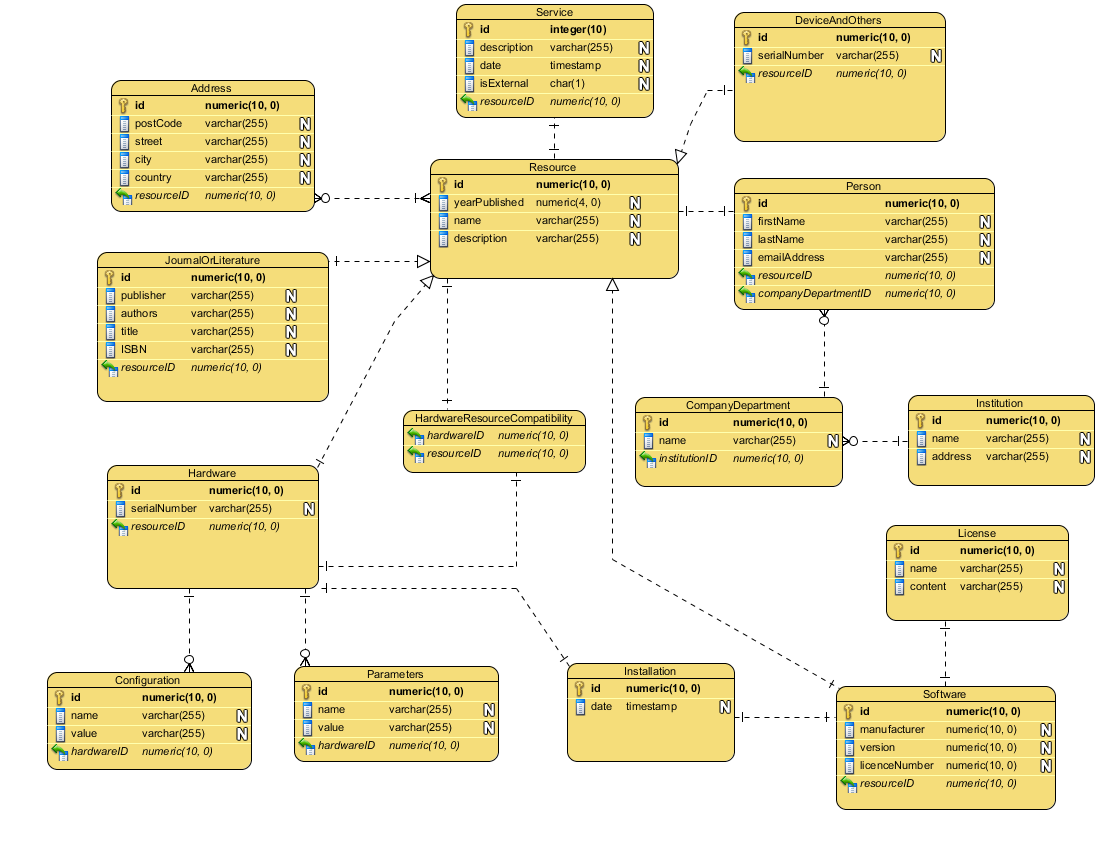
\includegraphics[scale=0.57, angle=270]{img/diagrams/LDM/LDM}
	\caption{Logiczny model danych\label{fig:labelLDM}}
\end{figure}
\bigskip
\subsection{Opis tabel}

\subsubsection{Address}
Odpowiada za przechowywanie adresu zasobu.
\begin{table}[H]
	\renewcommand\arraystretch{1.5}
	\renewcommand\tabcolsep{1.5pt}
\begin{tabular}{| c | c | c | c |} 
	\hline \textbf{Nazwa atrybutu} & \textbf{Znaczenie atrybutu} & \textbf{Typ danych} & \textbf{Ograniczenia} \\ 
	\hline ID & PRIMARY KEY & Numeric(10,0) & NOT NULL, UNIQUE \\ 
	\hline postCode & Kod pocztowy & Varchar(255) & REGEXP LIKE \\
	~ & ~ & ~ & \verb|[([0-9]\{2}-[0-9]\{3})| \\ 
	\hline street & Ulica & Varchar(255) &  \\ 
	\hline city & Miasto & Varchar(255) & \\ 
	\hline country & Kraj & Varchar(255) &  \\ 
	\hline resourceID & FOREIGN KEY & Numeric(10,0) & \\ 
	\hline 
\end{tabular}
\caption{Tabela Address}
\label{TAB:Address}
\end{table} 

\subsubsection{Service}
Przechowuje usługę serwisową.
\begin{table}[H]
	\renewcommand\arraystretch{1.5}
	\renewcommand\tabcolsep{1pt}
	\begin{tabular}{| c | c | c | c |} 
	\hline \textbf{Nazwa atrybutu} & \textbf{Znaczenie atrybutu} & \textbf{Typ danych} & \textbf{Ograniczenia} \\ 
	\hline ID & PRIMARY KEY & Numeric(10,0) & NOT NULL, UNIQUE \\ 
	\hline Description & Opis & Varchar(255) & \\ 
	\hline Date & Data & Timestamp &  \\ 
	\hline isExternal & Czy usługa została zlecona zewnętrznie? & Char(1) & \\ 
	\hline resourceID & FOREIGN KEY & Numeric(10,0) & \\ 
	\hline 
\end{tabular}
\caption{Tabela Service}
\label{TAB:Service}
\end{table} 

\subsubsection{Person}
Reprezentuje osobę (użytkownik, administrator).
\begin{table}[H]
	\renewcommand\arraystretch{1.5}
	\renewcommand\tabcolsep{3pt}
\begin{tabular}{| c | c | c | c |}
	\hline \textbf{Nazwa atrybutu} & \textbf{Znaczenie atrybutu} & \textbf{Typ danych} & \textbf{Ograniczenia} \\ 
	\hline ID & PRIMARY KEY & Numeric(10,0) & NOT NULL, UNIQUE \\ 
	\hline firstName & Imię & Varchar(255) & \\ 
	\hline lastName & Nazwisko & Varchar(255) &  \\ 
	\hline emailAddress & Adres email & Varchar(255) & REGEXP LIKE\\
	~ & ~ & ~ & \verb|[a-z0-9_.-]|\\ 
	~ & ~ & ~ & \verb|+@[a-z0-9_.-]|\\ 
	~ & ~ & ~ & \verb|+\.\ w {2,4}|\\ 
	\hline resourceID & FOREIGN KEY & Numeric(10,0) & \\ 
	\hline companyDepartmentID & FOREIGN KEY & Numeric(10,0) & \\ 
	\hline 
\end{tabular} 
\caption{Tabela Person}
\label{TAB:Person}
\end{table}

\subsubsection{CompanyDepartment}
Reprezentuje dział firmy.
\begin{table}[H]
	\renewcommand\arraystretch{1.5}
	\renewcommand\tabcolsep{3pt}
	\begin{tabular}{| c | c | c | c |} 
		\hline \textbf{Nazwa atrybutu} & \textbf{Znaczenie atrybutu} & \textbf{Typ danych} & \textbf{Ograniczenia} \\ 
		\hline ID & PRIMARY KEY & Numeric(10,0) & NOT NULL, UNIQUE \\ 
		\hline Name & Nazwa działu & Varchar(255) &  \\ 
		\hline institutionID & FOREIGN KEY & Numeric(10,0) & \\ 
		\hline 
	\end{tabular} 
	\caption{Tabela CompanyDepartment}
	\label{TAB:CompanyDepartment}
\end{table}

\subsubsection{CompanyDepartment}
Reprezentuje dział firmy.
\begin{table}[H]
	\renewcommand\arraystretch{1.5}
	\renewcommand\tabcolsep{3pt}
	\begin{tabular}{| c | c | c | c |} 
		\hline \textbf{Nazwa atrybutu} & \textbf{Znaczenie atrybutu} & \textbf{Typ danych} & \textbf{Ograniczenia} \\ 
		\hline ID & PRIMARY KEY & Numeric(10,0) & NOT NULL, UNIQUE \\ 
		\hline Name & Nazwa działu & Varchar(255) &  \\ 
		\hline institutionID & FOREIGN KEY & Numeric(10,0) & \\ 
		\hline 
	\end{tabular} 
	\caption{Tabela CompanyDepartment}
	\label{TAB:CompanyDepartment}
\end{table}

\subsubsection{Institution}
Reprezentuje oddział firmy.
\begin{table}[H]
	\renewcommand\arraystretch{1.5}
	\renewcommand\tabcolsep{3pt}
	\begin{tabular}{| c | c | c | c |} 
		\hline \textbf{Nazwa atrybutu} & \textbf{Znaczenie atrybutu} & \textbf{Typ danych} & \textbf{Ograniczenia} \\ 
		\hline ID & PRIMARY KEY & Numeric(10,0) & NOT NULL, UNIQUE \\ 
		\hline Name & Nazwa oddziału & Varchar(255) &  \\ 
		\hline Address & Adres & Varchar(255) & \\ 
		\hline 
	\end{tabular} 
	\caption{Tabela Institution}
	\label{TAB:Institution}
\end{table}

\subsubsection{License}
Reprezentuje licencję.
\begin{table}[H]
	\renewcommand\arraystretch{1.5}
	\renewcommand\tabcolsep{3pt}
	\begin{tabular}{| c | c | c | c |} 
		\hline \textbf{Nazwa atrybutu} & \textbf{Znaczenie atrybutu} & \textbf{Typ danych} & \textbf{Ograniczenia} \\ 
		\hline ID & PRIMARY KEY & Numeric(10,0) & NOT NULL, UNIQUE \\ 
		\hline Name & Nazwa & Varchar(255) &  \\ 
		\hline Content & Zawartość & Varchar(255) & \\ 
		\hline 
	\end{tabular} 
	\caption{Tabela License}
	\label{TAB:License}
\end{table}

\subsubsection{Installation}
Reprezentuje instalację (powiązanie software z hardware).
\begin{table}[H]
	\renewcommand\arraystretch{1.5}
	\renewcommand\tabcolsep{3pt}
	\begin{tabular}{| c | c | c | c |} 
		\hline \textbf{Nazwa atrybutu} & \textbf{Znaczenie atrybutu} & \textbf{Typ danych} & \textbf{Ograniczenia} \\ 
		\hline ID & PRIMARY KEY & Numeric(10,0) & NOT NULL, UNIQUE \\ 
		\hline Date & Data instalacji & timestamp &  \\ 
		\hline 
	\end{tabular} 
	\caption{Tabela Installation}
	\label{TAB:Installation}
\end{table}

\subsubsection{Configuration}
Reprezentuje konfigurację.
\begin{table}[H]
	\renewcommand\arraystretch{1.5}
	\renewcommand\tabcolsep{3pt}
	\begin{tabular}{| c | c | c | c |} 
		\hline \textbf{Nazwa atrybutu} & \textbf{Znaczenie atrybutu} & \textbf{Typ danych} & \textbf{Ograniczenia} \\ 
		\hline ID & PRIMARY KEY & Numeric(10,0) & NOT NULL, UNIQUE \\ 
		\hline Name & Nazwa konfigurowanej wartości & Varchar(255) &  \\ 
		\hline Name & Wartość & Varchar(255) &  \\
		\hline hardwareID & FOREIGN KEY & Numeric(10,0) & \\ 
		\hline 
	\end{tabular} 
	\caption{Tabela Configuration}
	\label{TAB:Configuration}
\end{table}

\subsubsection{Parameters}
Reprezentuje parametry (parametry i ich wartości).
\begin{table}[H]
	\renewcommand\arraystretch{1.5}
	\renewcommand\tabcolsep{3pt}
	\begin{tabular}{| c | c | c | c |} 
		\hline \textbf{Nazwa atrybutu} & \textbf{Znaczenie atrybutu} & \textbf{Typ danych} & \textbf{Ograniczenia} \\ 
		\hline ID & PRIMARY KEY & Numeric(10,0) & NOT NULL, UNIQUE \\ 
		\hline Name & Nazwa parametru & Varchar(255) &  \\ 
		\hline Name & Wartość & Varchar(255) &  \\
		\hline hardwareID & FOREIGN KEY & Numeric(10,0) & \\ 
		\hline 
	\end{tabular} 
	\caption{Tabela Parameters}
	\label{TAB:Parameters}
\end{table}